\section{State}

O State permite alterar o comportamento de um objeto baseado 
em seu estado interno. Uma interface define os comportamentos 
que dependem do estado do objeto e classes que a implementam 
definem a implementação dos mesmos. Dessa forma, o objeto 
principal delega as operações às classes que representam 
seu estado.

Esse padrão contribui para o reuso de operações comuns quando 
diversas classes relacionadas teriam que ser reinstanciadas 
durante uma mudança de estado. Também é permitido que o 
estado mude dinamicamente durante a execução.

\begin{figure}[htb]
	\caption{\label{state_struct}Estrutura do State}
	\begin{center}
	    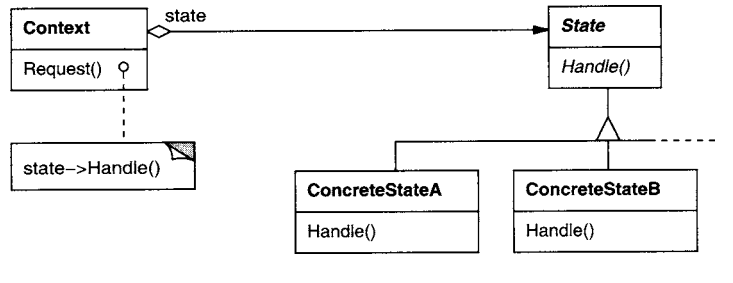
\includegraphics[scale=0.5]{5_padroes-contexto-funcional/5.3_comportamentais/5.3.08_state/diagram.png}
	\end{center}
\end{figure}

\subsection*{Exemplo Orientado a Objetos}

\begin{figure}[htb]
	\caption{\label{state_exemplo}Exemplo de State}
	\begin{center}
	    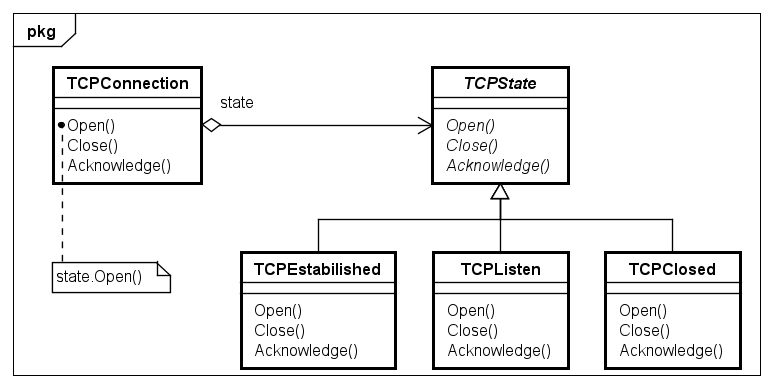
\includegraphics[scale=0.5]{5_padroes-contexto-funcional/5.3_comportamentais/5.3.08_state/state_exemplo.png}
	\end{center}
\end{figure}

\begin{lstlisting}[caption={State Orientação a Objetos},label=oostate]

trait State{
    def pressButton() : State
}

class OnState() extends State {
    def pressButton() : State = new OffState()
}

class OffState() extends State {
    def pressButton() : State = new OnState()
}

class Lamp(state : State) {
    def pressButton() : Unit {
        this.state = state.pressButton()
    }
}
    
\end{lstlisting}

\subsection*{Contexto Funcional}

\begin{comment}
Normalmente, a primeira alternativa que se tem em mente é 
o monad State. Porém, esse monad é focado em comportamentos 
que alteram o estado atual do nosso valor. Por mais que isso 
seja possível através do padrão State, por definição, sua 
intenção é fornecer comportamentos que não necessariamente 
altera o estado interno do valor.

Dessa forma, uma maneira interessante de definir o State 
no contexto funcional é utilizando uma case class que armazena, 
além dos valores comuns, um valor referente a um State. 
Esse State nada mais é do que outra clase class que 
irá armazenar, através de funções, os comportamentos que 
dependem de um estado. Da mesma forma que uma interface 
define as assinaturas das operações no exemplo orientado a 
objetos, aqui a definição da case class definirá que tipos 
de comportamentos a case class principal deverá possuir.

\begin{lstlisting}[caption={State Funcional},label=fpstate]
    
case class LampState(pressButton : () => Lamp)

case class Lamp(state : LampState)

def pressButton(lamp : Lamp) : Lamp =
    lamp.state.pressButton()

val onState : LampState = LampState(() => offState)

val offState : LampState = LampState(() => onState)
    
\end{lstlisting}

É importante notar que, aqui, quando o estado do valor 
principal precisa ser supostamente modificado, o que na 
verdade acontecerá é que a função da case class State 
irá retornar o nosso valor atualizado.

\end{comment}